\section*{Exercise 1}
\label{sec:exercise1}

\subsection*{Part A}

Using the minimax algorithm, we assume that both players play optimally (namely the MAX player maximizes his utility value, while the MIN player minimizes the same value). Furthermore, the algorithm performs a complete depth-first exploration of the corresponding game tree (Figure \ref{fig:exercise1}), assigning the minimum or maximum utility value out of all its children nodes as a minimax value to every MIN or MAX node respectively. 

In this case, MIN nodes B, C, D and E would be given the values -12, -7, -9, 2 respectively, while the starting MAX node will take the maximum of these four values, namely 2. Therefore, the resulting optimal move for the MAX player would lead to E, and the optimal response by the MIN player would then lead to the terminal node with utility value 2.

\subsection*{Part B}

Figure \ref{fig:exercise1} depicts the game tree.

\begin{figure}[htpb]
\centering
\makebox[\textwidth]{%
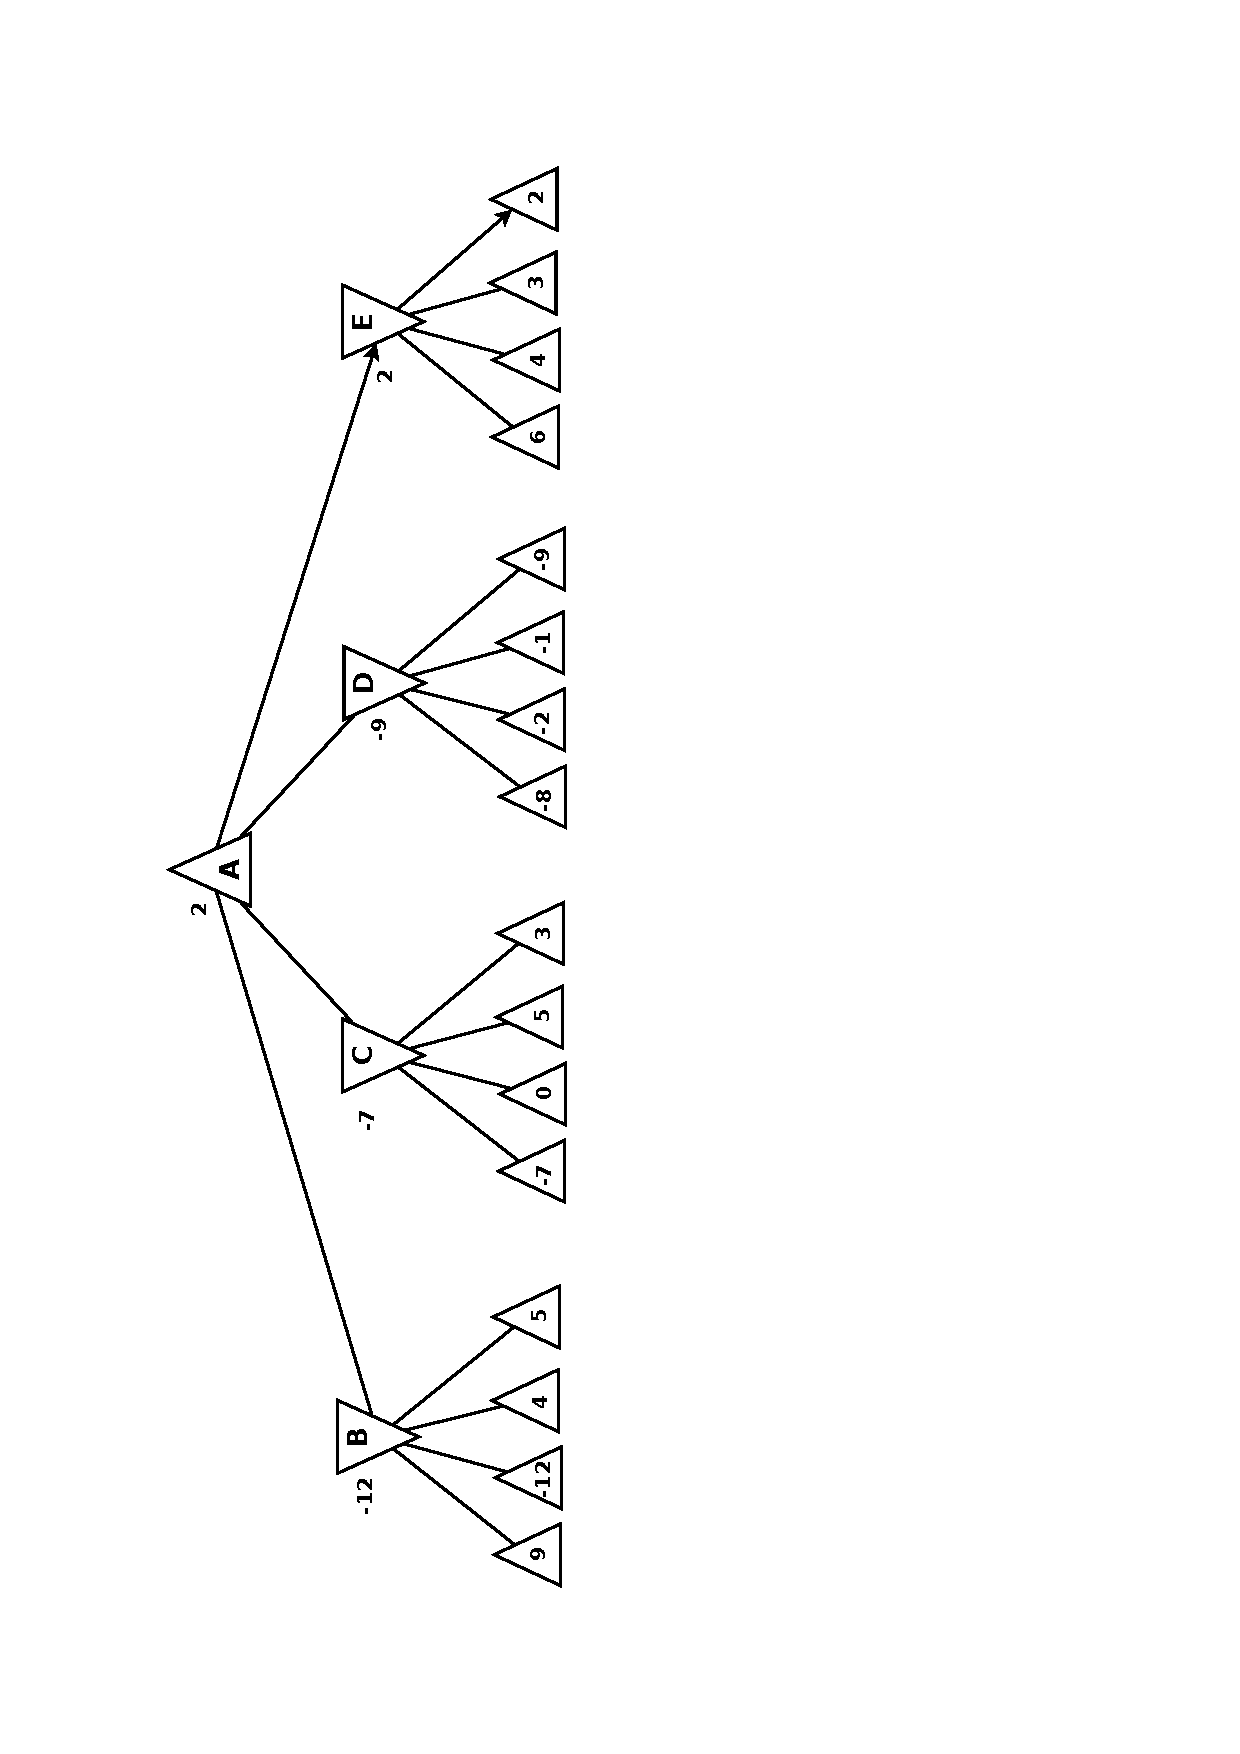
\includegraphics[width=0.3\textwidth, angle = -90, trim = 25mm 25mm 110mm 25mm,clip=true]{images/exercise1.pdf}}
\caption{The complete game tree of exercise 1. The $\bigtriangleup$ nodes represent MAX ones, whereas the $\bigtriangledown$ nodes represent MIN ones. The terminal nodes (leaves) show the utility values for MAX, whilst the other nodes are labeled with their minimax values.}
\label{fig:exercise1}
% Place the label just after the caption to make the link work
\end{figure} % table makes a floating object with a title

\section*{Exercise 2}

Given a binary mask $M$ and two parental solutions $A$ and $B$, their offspring $C$ produced by the genetic algorithm will inherit the value $A_i$ for each $M_i = 0$ and $B_j$ for each $M_j = 1$, where $i,j$ are indices of $A, B, M, C$. Therefore, for $A=00110101$ and $B=11010100$ the offsprings would be:

a) $ M=00000111 \Rightarrow C =  00110100$

b) $ M=00111000 \Rightarrow C = 00010101$

c) $ M=00110110 \Rightarrow C = 00010101$

\section*{Exercise 3}

\subsection*{Part A}

First, we need to consider that Part B requires a binary constraint satisfaction problem (CSP) because the AC-3 algorithm can only be used with binary constraints. Let $f(T_i)$ be the number of offices of department $T_i$, then the following observations lead to such a binary CSP formulation:

\begin{enumerate}

\item We can see from the data that $\sum_{i=1}^{12} f(T_i)=120$, in other words the company needs 120 offices in total. Given that each floor can provide at most 40 offices, each floor must have all its offices occupied (otherwise the sum of occupied offices will not be 120 and consequently not all departments will be housed).

\item Since each floor will have exactly 40 occupied offices, we can easily find the lower and upper bound for the number of departments per floor. By summing the offices of the three largest departments ($f(T_3)+f(T_4)+f(T_6)=36$), we deduce that each floor must have $\ge$4 departments. Moreover, if a floor houses $>$4 departments, then at least one floor must have $<$4 departments, which is a contradiction. Therefore, each floor will house exactly 4 departments.

\item We know that some departments should be on the same floor ($T_1$ with $T_3$, $T_2$ with $T_4$, $T_8$ with $T_9$). Since no combination of these pairs can occupy exactly 40 offices ($f(T_1)+f(T_3)+f(T_2)+f(T_4) = 39$, $f(T_1)+f(T_3)+f(T_8)+f(T_9) = 38$ and $f(T_2)+f(T_4)+f(T_8)+f(T_9) = 37$), we conclude that each pair should be assigned to a different floor.

\end{enumerate}

We are now able to define the binary CSP problem. Let $X_i \in \{T_5, T_6, T_7, T_{10}, T_{11}, T_{12}\}$, $i \in \{1, 2, 3, 4, 5, 6\}$ be the remaining departments to be allocated, then the binary constraints will be:

\[
	\begin{array}{ll}
		X_i \ne X_j, \forall (i,j) : i \ne j \\
		f(X_1) + f(X_2) + f(T_1) + f(T_3) = 40 \Rightarrow f(X_1) + f(X_2) = 20 \\
		f(X_3) + f(X_4) + f(T_2) + f(T_4) = 40 \Rightarrow f(X_3) + f(X_4) = 21 \\
		f(X_5) + f(X_6) + f(T_8) + f(T_9) = 40 \Rightarrow f(X_5) + f(X_6) = 22
	\end{array}
\]

\subsection*{Part B}

\begin{table}[htpb]
\centering
\makebox{
\resizebox{!}{1.95cm}{
\begin{tabular}{| c | c | p{3.7cm} | p{3.7cm} | p{3.7cm} |}
\hline
& Initial Domain & $(X_1 \ne X_2) \cap (f(X_1) + f(X_2) = 20)$ & $(X_3 \ne X_4) \cap (f(X_3) + f(X_4) = 21)$ & $(X_5 \ne X_6) \cap (f(X_5) + f(X_6) = 22)$\\
\hline
$X_1$ & $T_5, T_6, T_7, T_{10}, T_{11}, T_{12}$ & $T_5, T_7, T_{10}, T_{11}, T_{12}$ & $T_5, T_7, T_{10}, T_{11}, T_{12}$ & $T_5, T_7, T_{10}, T_{11}, T_{12}$ \\
\hline
$X_2$ & $T_5, T_6, T_7, T_{10}, T_{11}, T_{12}$ & $T_5, T_7, T_{10}, T_{11}, T_{12}$ & $T_5, T_7, T_{10}, T_{11}, T_{12}$ & $T_5, T_7, T_{10}, T_{11}, T_{12}$ \\
\hline
$X_3$ & $T_5, T_6, T_7, T_{10}, T_{11}, T_{12}$ & $T_5, T_6, T_7, T_{10}, T_{11}, T_{12}$ & $T_5, T_6, T_7, T_{10}, T_{11}, T_{12}$ & $T_5, T_6, T_7, T_{10}, T_{11}, T_{12}$ \\
\hline
$X_4$ & $T_5, T_6, T_7, T_{10}, T_{11}, T_{12}$ & $T_5, T_6, T_7, T_{10}, T_{11}, T_{12}$ & $T_5, T_6, T_7, T_{10}, T_{11}, T_{12}$ & $T_5, T_6, T_7, T_{10}, T_{11}, T_{12}$ \\
\hline
$X_5$ & $T_5, T_6, T_7, T_{10}, T_{11}, T_{12}$ & $T_5, T_6, T_7, T_{10}, T_{11}, T_{12}$ & $T_5, T_6, T_7, T_{10}, T_{11}, T_{12}$ & $T_6, T_7, T_{10}, T_{11}, T_{12}$ \\
\hline
$X_6$ & $T_5, T_6, T_7, T_{10}, T_{11}, T_{12}$ & $T_5, T_6, T_7, T_{10}, T_{11}, T_{12}$ & $T_5, T_6, T_7, T_{10}, T_{11}, T_{12}$ & $T_6, T_7, T_{10}, T_{11}, T_{12}$ \\
\hline
\end{tabular}
}}
\caption{The initial progress of the AC-3 algorithm for the first three (and their reverse) arcs. The columns contain the initial domain of each variable, and the updated domains after considering the first three (and their reverse) arcs of the queue.}
\label{table:ac3}
\end{table}

The aforementioned constraint equations contain 30 arcs in total (since all nodes of its undirected graph representation are connected with each other and arcs are directed). Assume that the initial queue of arcs given to AC-3 is $[(X_1 \ne X_2) \cap (f(X_1) + f(X_2) = 20), (X_3 \ne X_4) \cap (f(X_3) + f(X_4) = 21), (X_5 \ne X_6) \cap (f(X_5) + f(X_6) = 22), X_1 \ne X_3, X_1 \ne X_4, ..., X_4 \ne X_6]$. Then the first iteration of AC-3 is to remove the first arc (and its reverse) and check each value in the domain of $X_1$ (and $X_2$ respectively) for inconsistencies. The updated domain is then $X_1, X_2 \in \{T_5, T_7, T_{10}, T_{11}, T_{12}\}$. Since the domain of $X_1$ (the same applies for $X_2$) has been updated, each arc ($X_k$,$X_1$), $k\ne1$ need to be added in the queue for rechecking (in the first iteration all these arcs are already in the queue).

The following iterations continue in a similar fashion until either the queue (success) or a domain (failure) is empty. Table \ref{table:ac3} shows how the domain is updated for the first three (six if we count the reverse arcs separately) iterations of the algorithm.


\section*{Exercise 4}

As explained in Exercise 1, the minimax algorithm guarantees the optimal solution for the MAX player given that both players make optimal decisions. Assuming that the MIN player chooses a suboptimal action instead, then the value of the respective MIN node (and thus the resulting minimax value of its parental MAX node) cannot decrease because the optimal action already led to the minimum value. The same argument can inductively be expanded to the whole game tree, proving the assertion.

Giving an example, in Figure \ref{fig:exercise1} let the MIN player always select the second best available action. These suboptimal moves would then mean that the MAX player would receive 4, 0, -8 or 3 if he opted for B, C, D or E respectively. Since the optimal move found by minimax leads to E, the resulting value would increase from 2 to 3. However, moving to B would actually result in an even better value (4), thus illustrating that when the MAX player can predict a suboptimal play by MIN, there may be better strategies than following the minimax decision.


%\section*{Exercise 1}
%
%\subsection*{Part A}
%
%PEAS descriptions for a robot basketball player, industrial orange-apple sorter and a stock investor are given in Table \ref{table:peas}.
%
%\begin{table}[htpb]
\centering
\makebox{
\resizebox{!}{4cm}{\begin{tabular}{l p{5cm} p{5cm} p{5cm}}
\hline
\textbf{Agent Type} & Robot Basketball Player & Industrial Orange-Apple Sorter & Stock Investor \\
\hline
\up \textbox{\textbf{Performance} \\ \textbf{Measure}} & 

\begin{itemize}[leftmargin=*,noitemsep,topsep=0pt]
\item win \%
\item goals made / goals attempted \%
\item average points per game
\item performance index rating
\end{itemize} & 

\begin{itemize}[leftmargin=*,topsep=0pt,noitemsep]
\item accuracy \%
\item # fruits per second
\end{itemize} & 

\begin{itemize}[leftmargin=*,topsep=0pt,noitemsep]
\item average ROI
\item total earnings (or losses)
\item earnings per month/year
\end{itemize} \\
\hline
\up \textbf{Environment} &

\begin{itemize}[leftmargin=*,topsep=0pt,noitemsep]
\item basketball court
\item other agents (teammates and opponents)
\end{itemize} & 

\begin{itemize}[leftmargin=*,topsep=0pt,noitemsep]
\item conveyor belt and surrounding parts of engine
\item reception of sorted fruits (holes, boxes)
\end{itemize} & 

\begin{itemize}[leftmargin=*,topsep=0pt,noitemsep]
\item online stock markets
\item other agents (investors)
\end{itemize} \\
\hline
\up \textbf{Actuators} & & & \\
\hline
\up \textbf{Sensors} & & & \\
\hline
\end{tabular}}
}
\caption{������� ����� ������� ���������� ��� ����� ��� $�$ ����������� ���� �������.}
\label{table:peas}
\end{table}
%
%
%\subsection*{Part B}
%
%Table \ref{table:environments} contains the environmental characteristics of the three aforementioned agent types. In the following paragraphs I select a suitable agent design, providing a brief explanation for each agent type.
%
%
%\begin{table}[htpb]
\centering
\makebox{
\resizebox{!}{3.4cm}{\begin{tabular}{l p{5cm} p{5cm} p{5cm}}
\hline
\textbf{Characteristic} & Robot Basketball Player & Industrial Orange - Apple Sorter & Stock Investor \\
\hline
\up \textbox{\textbf{Observable}} & partial (court not entirely observable) & partial (e.g. fruit not entirely observable internally) & partial (too many markets, stocks and investors)   \\
\hline
\up \textbf{Determinism} & stochastic (e.g. shot/pass curve) & stochastic (e.g. photo background) & deterministic* (it depends on how the affecting sociopolitical conditions are modeled)/ strategic (during negotiations against other agents) \\
\hline
\up \textbf{Dependency} & sequential & episodic (each fruit checked separately) & sequential \\
\hline
\up \textbf{Dynamicity} & dynamic & semidynamic (fruit type does not change but performance depends on time) & dynamic (stock prices and financial conditions can fluctuate too rapidly to be considered static) \\
\hline
\up \textbf{Description} & continuous & continuous & continuous \\
\hline
\up \textbf{Cardinality} & multiagent & single agent & multiagent\\
\hline
\end{tabular}}
}
\caption{Characteristics of the environment of three agent types.}
\label{table:environments}
\end{table}
%
%\textbf{Robot basketball player:} \textit{Simple reflex agents} cannot perform well in this partially observable, dynamic environment. An \textit{internal-state model} could be used, but we would need many states that are difficult to define in such a continuous-state environment. In addition, simply storing the current state of the system would not be enough for the player to decide its next course of action. Furthermore, a \textit{goal-based agent} would be inefficient since scoring is not the only goal in basketball. Therefore, \textit{a utility-based model} is deemed necessary to provide a more efficient performance measure in this multiagent environment. Online \textit{learning} could also be applied during the match, allowing adaptation against the opposing team. Its application however would be difficult without sacrificing (at least their initial) performance.
%
%\textbf{Industrial orange-apple sorter:} An \textit{internal-state model} would be enough for fruit classification based on the partially observable fruits and stochastic background (e.g. varying light in the room or existing branches/leaves). \textit{Learning} would be useful if we wanted our agent to classify more types of fruits in the future.
%
%\textbf{Stock investor:} Similar to a robot basketball player, this agent needs to consider not only its basic goal of maximizing its net profit (namely buying cheaply and selling expensively), but also other features such as credibility, financial forecasts and cooperation with other investors. Therefore, a \textit{utility-based agent} would again be more appropriate. \textit{Learning} could also be proven useful in adaptation against opposing agents and new financial, cultural and political conditions.
%
%
%
%\section*{Exercise 2}
%
%\subsection*{Part A}
%
%The solution is given in Figure \ref{fig:exercise2}.
%
%\begin{figure}[htpb]
%\centering
%\makebox[\textwidth]{%
%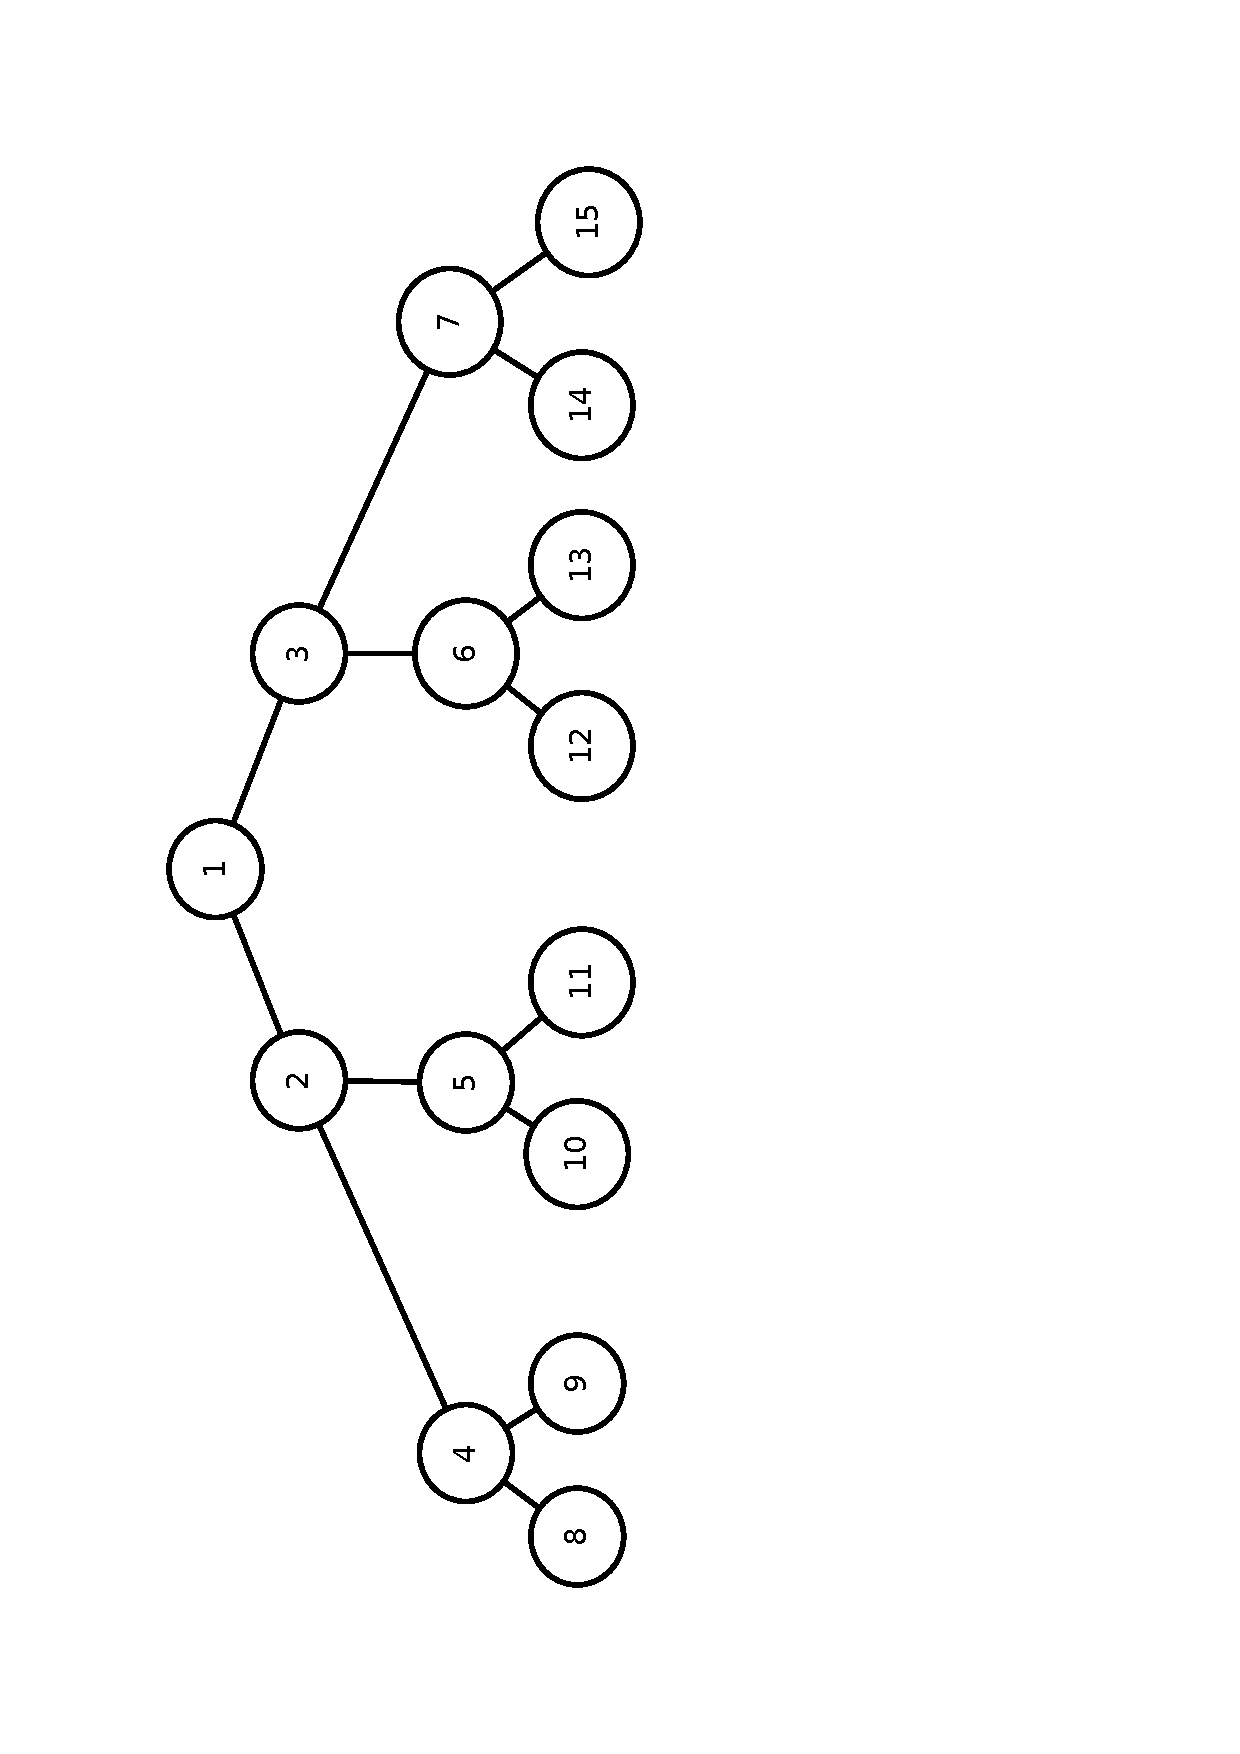
\includegraphics[width=0.3\textwidth, angle =-90, trim = 25mm 25mm 100mm 25mm,clip=true]{images/exercise2.pdf}}
%\caption{State space for states 1 to 15, starting from 1, while the successor function returning two states, $2n$ and $2n+1$.}
%\label{fig:exercise2}
%% Place the label just after the caption to make the link work
%\end{figure} % table makes a floating object with a title
%
%\subsection*{Part B}
%
%The order in which the nodes will be visited for each type of search is given below:
%
%\begin{itemize}
%
%\item Breadth-First Search: 1, 2, 3, 4, 5, 6, 7, 8, 9, 10, 11
%
%\item Depth-Limited Search (depth limit 3): 1, 2, 4, 8, 9, 5, 10, 11
%
%\item Iterative Deepening Search: (depth limit 0) 1 - (depth limit 1) 1, 2, 3 - (depth limit 2) 1, 2, 4, 5, 3, 6, 7 - (depth limit 3) 1, 2, 4, 8, 9, 5, 10, 11
%
%\end{itemize}
%
%\subsection*{Part C}
%
%Bidirectional search would be quite appropriate for this problem, since we could easily employ the inverse of the successor function for searching in the opposite direction (from goal to start state): $\lfloor n/2 \rfloor$. For example, the bidirectional search algorithm would work as follows:
%
%\begin{itemize}
%
%\item Search from start: 1, 2, 3
%
%\item Search from goal: 11, 5, (2)
%
%\end{itemize}
%
%The algorithm would terminate when the search from goal reaches node 2, which would have already been reached by the search from start. The final solution would therefore be 1, 2, 5, 11.
%
%Simple search from goal to start would actually allow us to avoid searching altogether because each node has only a single predecessor. Hence, the solution could simply be found in $\log_2{n}$ steps.
%
%\section*{Exercise 3}
%
%The solution is given in Figure \ref{fig:exercise3}.
%
%\begin{sidewaysfigure}[htpb]
%\centering
%\makebox[\textwidth]{%
%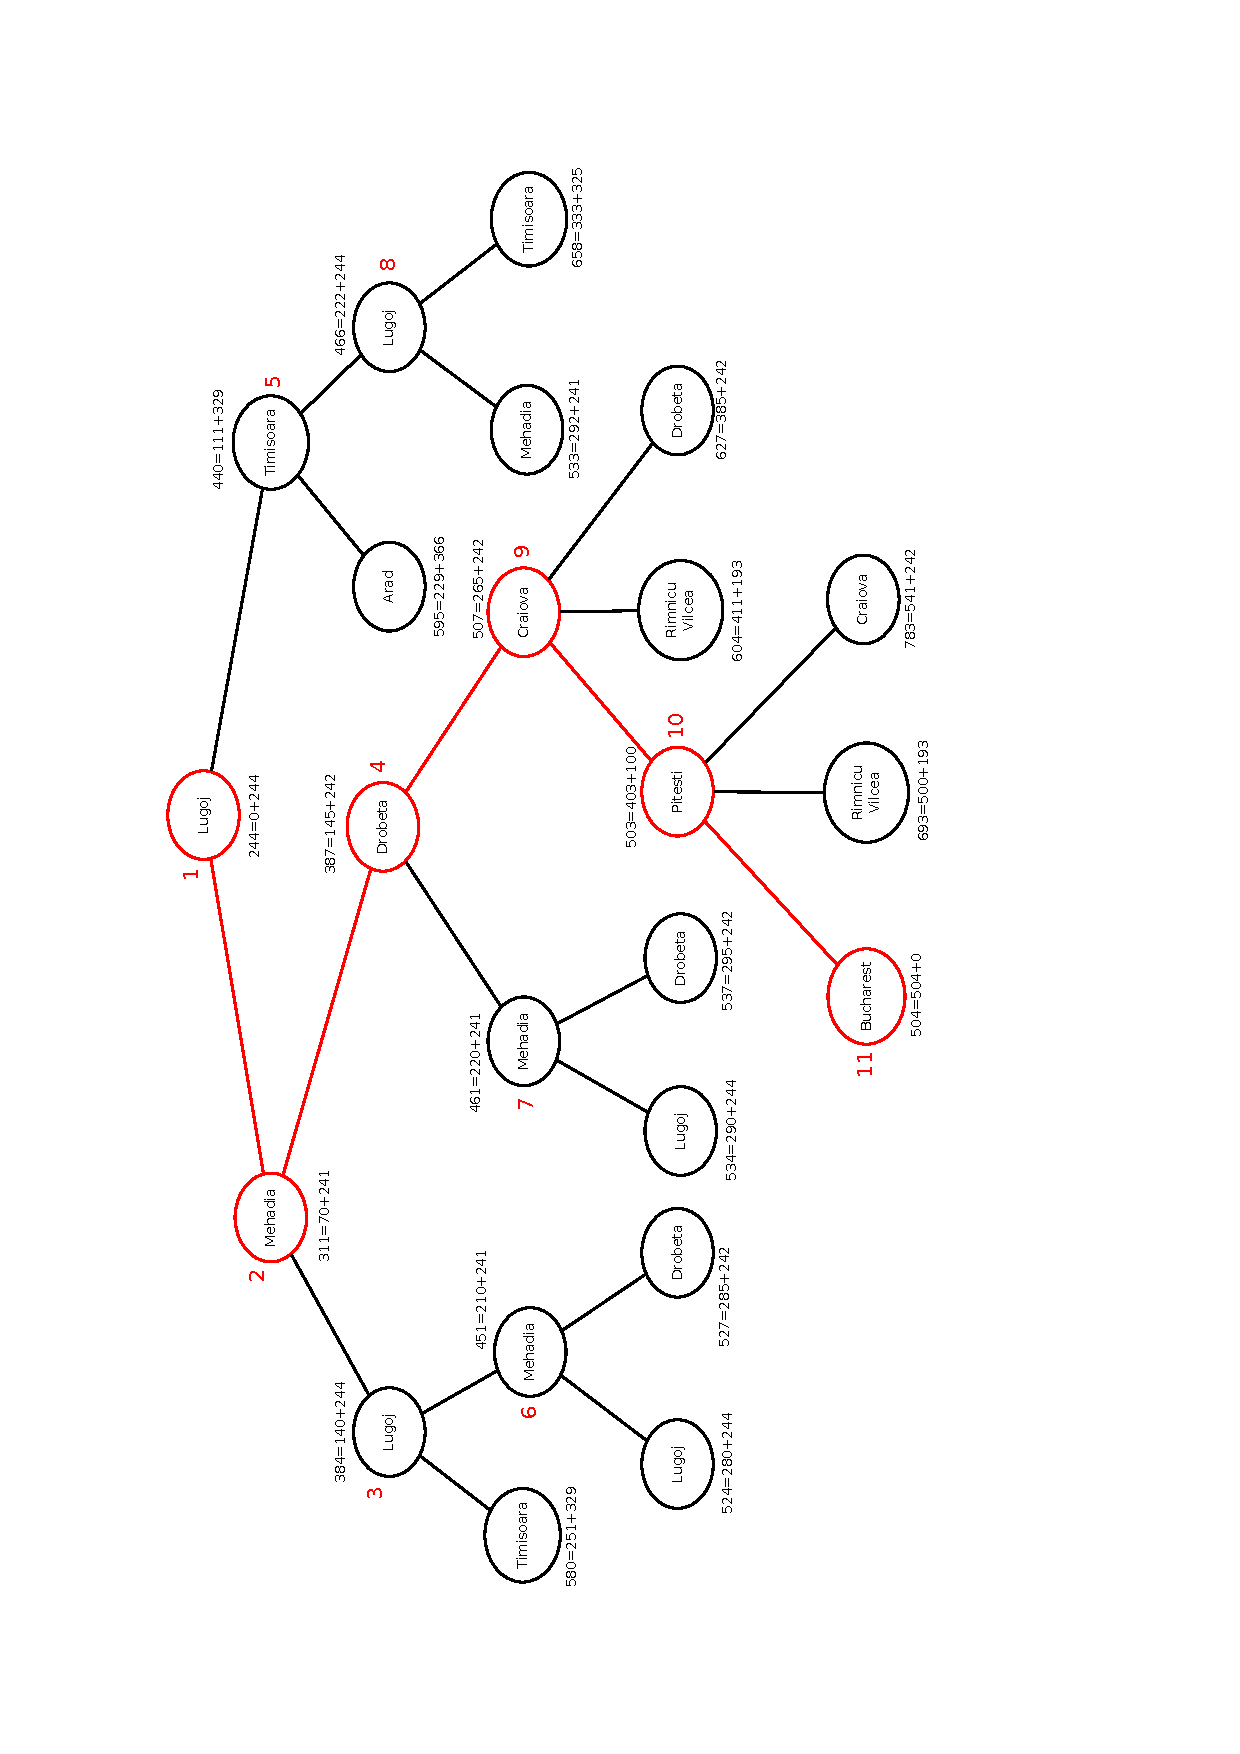
\includegraphics[width=0.55\textwidth, angle =-90, trim = 25mm 25mm 50mm 25mm,clip=true]{images/exercise3.pdf}}
%\caption{Stages in an A* search from Lugoj to Bucharest. Nodes are labeled with $f = g+ h$ (black font), and with the selected order of expansion (red font). The sequence of states that are considered during each iteration consists of the current leaf nodes. The algorithm expands the leaf node with the lowest value of $f$, replacing it in the sequence with all its successors (to be considered for the following iteration). The optimal solution is depicted with red nodes and edges.}
%\label{fig:exercise3}
%% Place the label just after the caption to make the link work
%\end{sidewaysfigure} % table makes a floating object with a title
%
%
%\section*{Exercise 4}
%
%\subsection*{Part A}
%
%Since only one state ($k=1$) is stored in memory after each iteration, it is iteratively succeeded by its best neighboring state like in hill climbing. Hence, the local beam search algorithm with $k=1$ is a simple hill climbing algorithm.
%
%\subsection*{Part B}
%
%With temperature $T=0$, we can say that the probability $e^{\Delta E/T}=0$ when $\Delta E \le 0$, namely only better neighboring solutions are accepted. Therefore, simulated annealing with $T=0$ is a first choice hill climbing algorithm.
%
%\subsection*{Part C}
%
%If $N=1$, the population will consist of a single individual. Crossover will thus happen between (two copies of) that individual, resulting in the exact same solution. The random mutation mechanism will introduce a small number of point changes during each iteration, consequently turning genetic algorithm into a random walk.






